\chapter{Conversione AD e convertitori - parte III}

\begin{figure}[h]
    \centering
    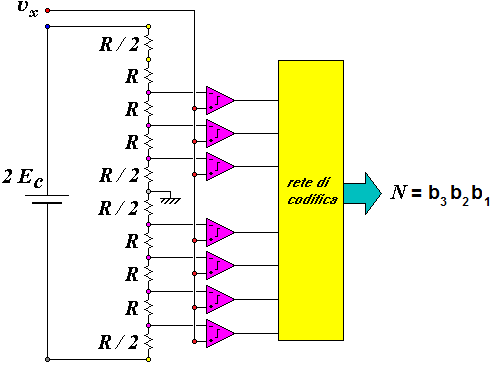
\includegraphics[scale = 1]{FLASH ADC.png}
\end{figure}

\newpage 

\section{Convertitori A / D}
\footnote{Slide della prof | SDME 3.Conversione AD e Convertitori - Parte III | pag 3 \\  
Appunti | 2025-03-28 | pag 2 - 3}

Il problema maggiore della conversione del segnale analogico digitale è il tempo di elaborazione, 
che deve essere minore del tempo indicato nel teorema del campionamento. \newline 

Con l'avanzare della tecnologia, il tempo di elaborazione è diminuito grazie ad architetture di A/D sempre più sofisticate e più efficienti. \newline 

A rigore, ci dovrebbero essere due dispositivi dopo la quantizzazione del segnale: quantizzatori e poi codificatori, 
ma per semplicità li consideriamo insieme e prendono il nome di convertitori A/D. \newline

\newpage 

\section{Convertitori paralleli "Flash ADC"}
\footnote{Slide della prof | SDME 3.Conversione AD e Convertitori - Parte III | pag 4 \\  
Appunti | 2025-03-28 | pag 4}

La prima tipologia di convertitori ADC sviluppati sono gli ADC Flash. \newline 

Un esempio di architettura ADC flash a 3 bit: 

\begin{figure}[h]
    \centering
    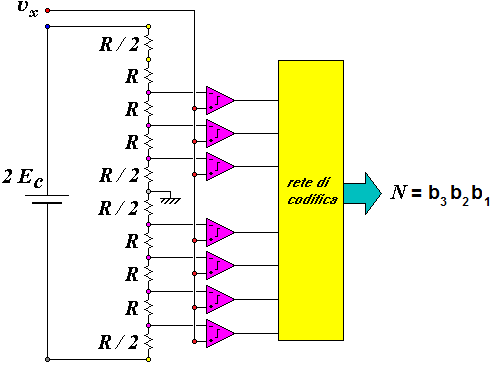
\includegraphics[scale = 0.8]{FLASH ADC.png}
\end{figure}

Sapendo che, per i motivi precedentemente elencati, svolgeremo una quantizzazione silenziata bipolare, 
tra $-E_c$ e $+E_c$, l'obbiettivo dell'architettura flash ADC è quello di dividere il campo di misura in un certo numero di intervalli contigui, 
individuando le frontiere tra questi. \newline 

Ad ogni campione si da il valore che corrisponde al valore centrale. \newline 

Analizzando il circuito del flash ADC, a sinistra notiamo che un campione di fem eroga una tensione pari a $2E_c$, che è proprio l'ampiezza del campo di misura bipolare. \newline 

$2E_c$ viene suddiviso in una rete di resistenze tutte uguali, tranne agli estremi. \newline 

$2E_c$ deve essere compatibile con il livello che bisogna misurare. \newline 

Le tensioni alle frontiere tra gli intervalli di quantizzazione sono le tensioni alle quali si trovano i nodi delle rete di resistenze. \newline 

Di seguito il circuito con gli appunti presi a lezione: 

\begin{figure}[h]
    \centering
    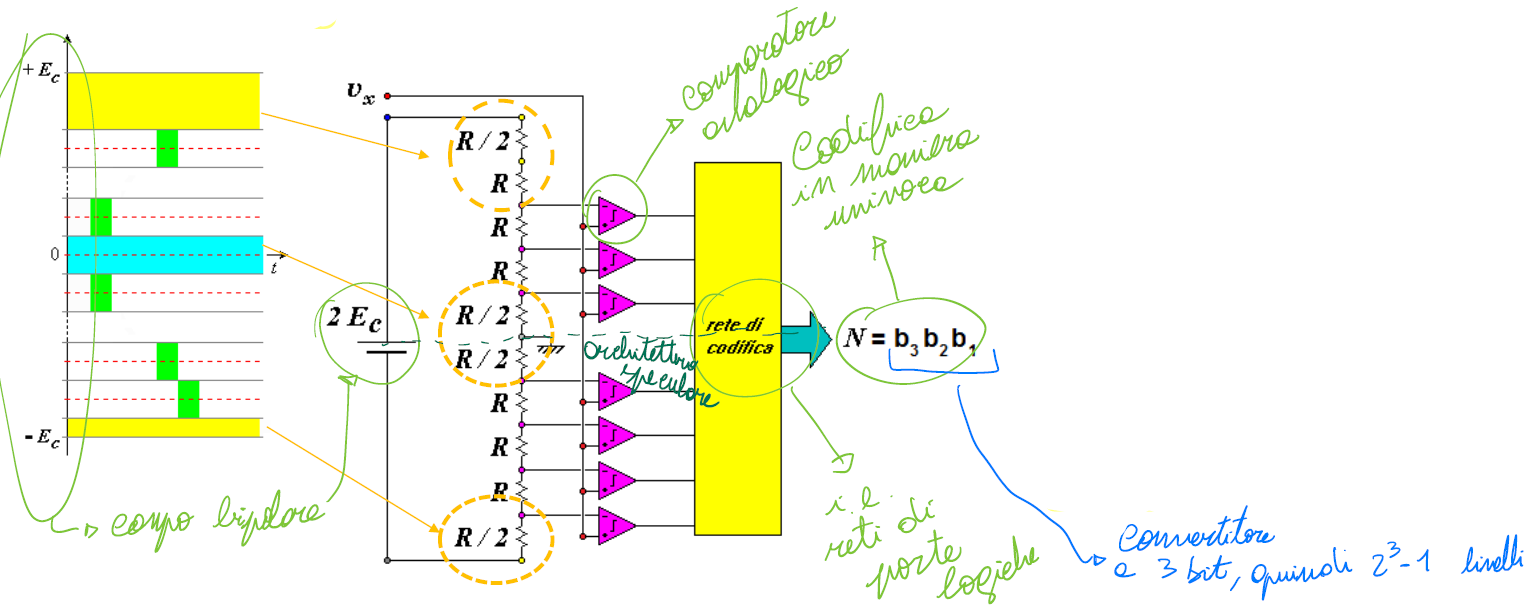
\includegraphics[scale = 0.6]{FLASH ADC con appunti.png}
\end{figure}

\newpage 

Il punto di forza di questa architettura è la semplicità concettuale perchè è composta solo da: 

\begin{itemize}
    \item una rete resistiva, per individuare le frontiere degli intervalli di quantizzazione 
    \item una rete di comparatori, per confrontare il valore della tensione di ingresso $v_x$ e la tensione di un nodo del resistore 
    \item una rete di codifica, che associa ad ognuna delle configurazioni di uscite dei comparatori una parola binaria in uscita in modo univoco
\end{itemize}

\newpage

\subsection{Flash ADC - Quantizzazione}
\footnote{Slide della prof | SDME 3.Conversione AD e Convertitori - Parte III | pag 7 - 8\\  
Appunti | 2025-03-28 | pag 5 - 8 }

\begin{figure}[h]
    \centering
    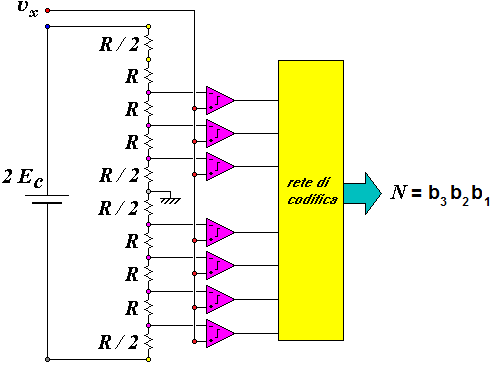
\includegraphics[scale = 0.5]{FLASH ADC.png}
\end{figure}

La tensione ad ogni nodo (rosso) viene portata in ingresso ad un comparatore (triangolini viola), 
il quale confronta la tensione del nodo e la tensione $v_x$ (campionata) da convertire. \newline 

Il comparatore analogico ci dice se il segnale posto ad uno dei due ingressi è maggiore di quello applicato all'altro ingresso. \newline 

Le uscite dei comparatori vengono messe in ingresso ad una rete di codifica. \newline 

La rete di codifica permette di avere in uscita una parola binaria (quella indicata nella figura con N), 
che rappresenta l'intervallo entro cui i comparatori hanno individuato che si trova la tensione $v_x$. \newline 

L'architettura flash ADC è veloce proprio perchè ogni comparatore lavora autonomamente. \newline 

Analizzando la figura dell'architettura di esempio, il campo di misura viene diviso in 8 intervalli, quindi la parola codificata in una parola di 3 bit perchè: 

{
    \Large 
    \begin{equation}
        \text{Numero intervalli} = 2^{3} = 8
    \end{equation}
}

La tensione ai capi della resistenza R è l'ampiezza dell'intervallo di quantizzazione, 
quindi è legata all'incertezza. \newline 

Teoricamente, per ridurre l'incertezza, bisognerebbe aggiungere più resistori in serie, in modo da suddividere il campo di misura 
in un maggior numero di intervalli. \newline 

Il Sample and Hold ha prelevato il livello di tensione $v_x$, ma non l'ha misurata: 
è compito dell'ADC codificare quel livello. \newline 

Supponiamo che $v_x$ si trova nel seguente intervallo (tra il punto 1 e il punto 2): 

\begin{figure}[h]
    \centering
    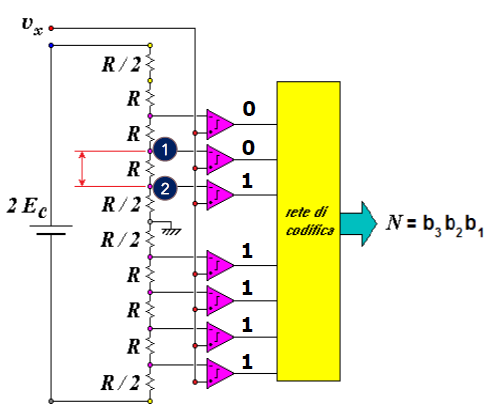
\includegraphics[scale = 0.5]{Flash ADC con Vx tra due resistori.PNG}
\end{figure}

$v_x$ è maggiore del valore di tensione al nodo 2 e minore del valore di tensione al nodo 1. \newline 

In formule: 

{
    \Large 
    \begin{equation}
        v_2 < v_x < v_1
    \end{equation}
}
Noi sappiamo che $v_x$ è compreso tra $v_1$ e $v_2$, ma non sappiamo quanto vale "realmente" $v_x$: 
se il nuovo $v_x ^{'}$ sarà compreso tra $v_1$ e $v_2$, dal codificatore uscirà la stessa parola di $v_x$. \newline 

Il comparatore collegato al nodo 2 avrà un'uscita a 1: 
l'ingresso invertente si trova a una tensione più bassa dell'ingresso non invertente. \newline 

Questo accade per tutti i comparatori "sotto" a questo, quindi avranno un'uscita al livello alto (cioè ad 1). \newline 

Il compratore collegato al nodo 1, avrà uscita a 0: 
la tensione in ingresso invertente è maggiore di quella all'ingresso non invertente. \newline 


La rete di codifica deve individuare qual è la posizione della frontiera tra le uscite a 1 le uscite a 0 dei comparatori, 
ovvero ha bisogno di individuare in quale intervallo si trova la tensione $v_x$ e fornisce in uscita una parola binaria che ne codifichi il valore in modo univoco. \newline 

\newpage 

\subsection{Flash ADC - codifica}
\footnote{Slide della prof | SDME 3.Conversione AD e Convertitori - Parte III | pag 9 - 10 \\  
Appunti | 2025-03-28 | pag 5 - 6, 8}

Considerando l'esempio: 

\begin{figure}[h]
    \centering
    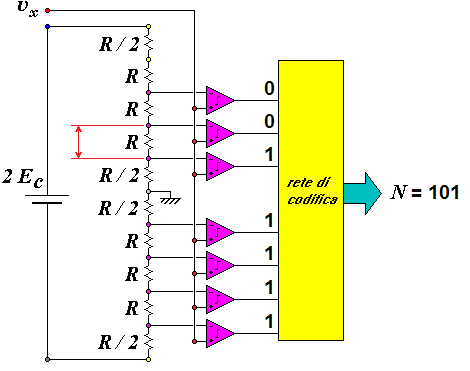
\includegraphics[scale = 0.5]{Flash ADC con parola di esempio.png}
\end{figure}

La parola: 

{
    \Large 
    \begin{equation}
        N = 101
    \end{equation}
}

è la parola binaria che individua in modo univoco la tensione $v_x$. \newline 

Si può utilizzare qualsiasi tipo di codifica, quindi far corrispondere il livello di tensione $v_x$ a una parola di codice N. \newline 

In particolare, sono necessarie due parole di codice: 

\begin{itemize}
    \item una di overflow, che la rete di codifica può indicare con i bit tutti a uno (nell'esempio a 3 bit 111) 
    \item una di underflow, che la rete di codifica può indicare con i bit tutti a zero (nell'esempio a 3 bit 000)
\end{itemize}

Nell'architettura flash ADC non è presente un buffer di memoria, quindi l'ADC deve convertire il segnale sotto al tempo di campionamento. \newline 

Qualunque valore della $v_x$ che si trovi a cadere tra valori della tensione di riferimento individuati dai nodi 1 e 2 verrà ad assumere la stessa codifica 
e questo darà a luogo a perdita di informazione, che a sua volta comporterà incertezza di quantizzazione. \newline 

L'architettura flash, non solo è veloce, ha una estrema rapidità di conversione grazie ai suoi pochi componenti. \newline 

L'unico "collo di bottiglia", per quanto riguarda il tempo, dell'architettura flash è la rete di codifica. \newline 

Il tempo di conversione è denominato dalla latenza della rete di codifica e tale tempo è comunemente breve. \newline 

L'aspetto negativo dell'architettura flash ADC è una incertezza di quantizzazione relativamente elevata quando si deve suddividere il campo di misura in un numero molto elevato di intervalli. \newline 

Si ha questa incertezza di quantizzazione molto elevata perchè sono presenti molti resistori e ognuno di essi contribuisce all'incertezza di quantizzazione. \newline 

Inoltre, aumentare il numero di bit non è possibile perchè un ADC flash a 8 bit richiede una rete di 256 resistori e 255 comparatori. \newline 

Questi limiti tecnologici limitano le prestazioni in termini di incertezza, che non sono trascurabili. \newline 

\newpage 

\subsection{Flash ADC - Codifica errori OF e UF}
\footnote{Slide della prof | SDME 3.Conversione AD e Convertitori - Parte III | pag 11 - 12 \\  
Appunti | 2025-03-28 | pag 8}

Come scritto precedentemente, l'architettura Flash ADC è molto importante perchè la rete di codifica segnala quando 
è presente un underflow (UF) o un overflow (OF). \newline 

Come si nota dalla seguente figura: 

\begin{figure}[h]
    \centering
    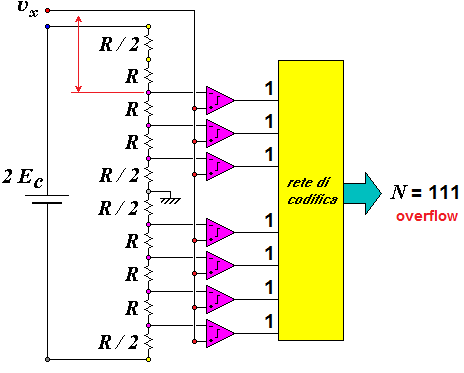
\includegraphics[scale = 0.8]{Flash ADC con overflow.png}
\end{figure}

abbiamo un caso di overflow, cioè la tensione di ingresso $v_x$ supera quella del nodo del terzo resistore R. \newline 

Tutti i comparatori segnano un'uscita a livello alto (cioè 1). \newline 

La rete di codifica segnala un errore di conversione e di overflow, ad esempio con la parola 111. \newline 

Invece, analizzando un caso di underflow: 

\begin{figure}[h]
    \centering
    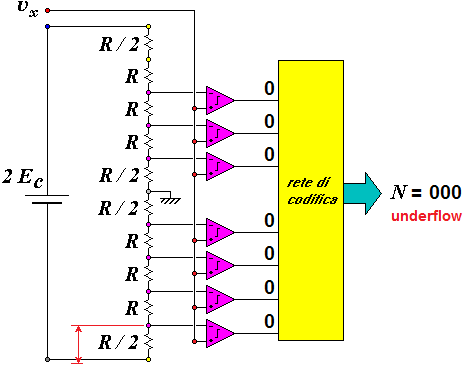
\includegraphics[scale = 0.8]{Flash ADC con underflow.png}
\end{figure}

succede il caso opposto dell'overflow. \newline 

La tensione di ingresso $v_x$ è al di sotto di quella minima. \newline 

Se la tensione $v_x$ è minore della tensione dell'ultimo nodo dell'ultimo resistore di valore $\frac{R}{2}$, 
allora la rete di codifica segnala la parola di underflow, ad esempio ponendo tutti i bit a 0. \newline 

Nel caso di esempio dei 3 bit, esiste UF con 000. \newline 

Come il caso dell'overflow, non sappiamo quando vale "realmente" $v_x$, sappiamo solo che è minore del campo di misura. \newline 


\newpage 

\subsection{Flash ADC: pro e contro}
\footnote{Slide della prof | SDME 3.Conversione AD e Convertitori - Parte III | pag 13 \\  
Appunti | 2025-03-28 | pag 8 - 9}

Per riassumere, di seguito i pro e i contro dell'architettura Flash ADC. \newline 

Il pro è la rapidità di conversione: generalmente è di 5 ns per 8 bit. \newline 

Il contro è l'elevata incertezza di quantizzazione, che è limitato dal numero di componenti da aggiungere, quindi il prezzo economico elevato 
dovuto all'aggiunta di ogni componente. \newline 

\newpage 

\section{Half-flash o semi-flash ADC}
\footnote{Slide della prof | SDME 3.Conversione AD e Convertitori - Parte III | pag 14 - 16 \\  
Appunti | 2025-03-28 | pag 9 - 10}

L'architettura Flash ha un enorme vantaggio, cioè la rapidità, ma ha un'elevata incertezza. \newline 

Per questo motivo, si è cercato di ovviare a ciò realizzando delle architetture più efficienti. \newline 

Gli ADC flash sono stati prima affiancati e poi sostituiti dai semi-flash. \newline 

Di seguito il block diagram di un half-flash ADC in commercio nel 1994: 

\begin{figure}[h]
    \centering
    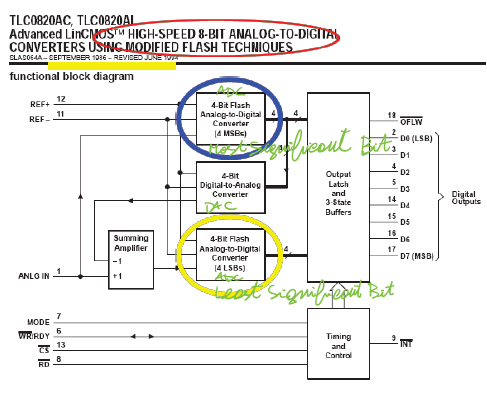
\includegraphics[scale = 1]{Esempio di Half-flash ADC.PNG}
\end{figure}

Un half-flash è un convertitore flash con una tecnica modificata, evidenziata dai 3 blocchi. \newline 

I blocchi estremi (quelli cerchiati in blu e in giallo) sono due convertitori flash a 4 bit ognuno, quindi: 

{
    \Large 
    \begin{equation}
        4 \text{bit flash ADC} + 4 \text{bit flash ADC} = 8 \text{bit half-flash ADC} 
    \end{equation}
}

Questi due ADC flash sono poi collegati ad un convertitore digitale/analogico a 4 bit. \newline 

Questi tre componenti sono poi collegati ad una rete combinatoria con capacità di memoria, in questo caso con un buffer a 3 stati. \newline 

Possiamo schematizzare i tre componenti più importanti degli half-flash ADC anche in questa maniera: 

\begin{figure}[h]
    \centering
    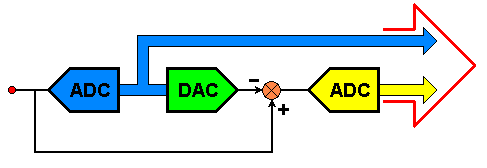
\includegraphics[scale = 1]{Half-flash ADC architettura.png}
\end{figure}

\newpage 

Di seguito la spiegazione completa del processo di conversione considerando un half-flash a 8 bit. \newline 

Un primo convertitore A/D a 4 bit (quello di colore blu in figura)  fa una prima conversione grossolana del segnale già campionato 
che ha in ingresso, avendo solo 16 livelli di quantizzazione perchè: 

{
    \Large 
    \begin{equation}
        4 \text{ bit} = 2^{4} = 16 \text{ livelli di quantizzazione} 
    \end{equation}
}

I 4 bit generati dalla rete di codifica dell'ADC flash vengono portati in uscita e sono i 4 bit più significativi della parola di uscita (alche nel block diagram è indicato come 4 MSBs). \newline 

Questi 4 bit vengono mandati al buffer e al convertitore digitale / analogico (quello indicato in verde): 
la tensione generata dal DAC è il valore centrale dell'intervallo al quale il campione di segnale è stato convertito e quantizzato dal primo convertitore. \newline 

La tensione "ricostruita" dal DAC viene sottratta alla tensione analogica in ingresso (nodo di sottrazione di colore arancione in figura). \newline 

In uscita dal nodo differenza, troviamo quello che possiamo chiamare il resto della prima conversione, cioè la differenza tra il valore del segnale di ingresso da convertire e la tensione che corrisponde al punto centrale dell'intervallo, in cui esso è stato convertito. \newline 

Tale ingresso è messo in ingresso ad un secondo convertitore A / D a 4 bit (quello che in figura è di colore giallo), 
ma che ha un campo di misura limitato all'ampiezza di un intervallo di quantizzazione (a differenza del primo ADC che ha due intervalli di quantizzazione). \newline 

Il resto non potrà essere maggiore di $\pm$ la metà dell'intervallo di quantizzazione del primo ADC. \newline 

Il resto viene convertito fornendo i 4 bit meno significativi della parola in uscita: alche nel block diagram dell'half-flash di esempio, 
il secondo ADC è indicato con la dicitura 4 LSBs. \newline 


Questo schema di principio sembra contraddittorio: perchè mettere due ADC in cascata con un DAC in mezzo tra loro ? \newline 

Il motivo è che sia gli ADC flash che i DAC sono molto semplici da realizzare. \newline 

\newpage 


\subsection{DAC a scala di resistenze}
\footnote{Slide della prof | SDME 3.Conversione AD e Convertitori - Parte III | pag 17 \\  
Appunti | 2025-03-28 | pag 10}

\begin{tcolorbox}
    Lo schema del principio del DAC a scala di resistenze lo chiede all'esame con gli esempi dei valori numerici
\end{tcolorbox}


Di seguito lo schema di principio di un DAC a scala di resistenze a 4 bit: 

\begin{figure}[h]
    \centering
    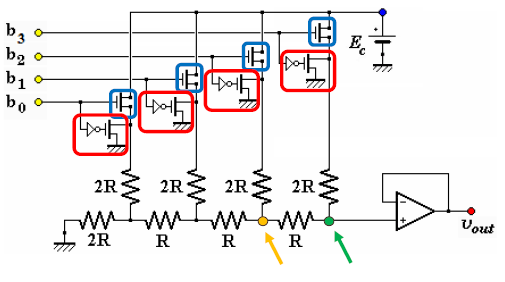
\includegraphics[scale = 1]{DAC a scala di resistenze 4 bit.PNG}
\end{figure}

In linea di principio, un convertitore D/A a 4 bit può essere realizzato con la componentistica mostrata. \newline 

Occorre avere un campione di fem (quello a destra nella figura indicato con $E_c$), 
che può essere applicata agli ingressi della rete resistiva nel caso in cui i MOS-FET (quelli cerchiati in blu) siano in conduzione (cioè si comportano idealmente da interruttore chiuso) e gli altri MOS-FET (quelli cerchiati di rosso) siano interdetti (cioè idealmente si comportano da interruttori aperti). \newline 

Se il bit $b_3$ è 1, il MOS-FET collegato alla sua linea conduce, 
e la tensione $E_c$ viene portata al nodo verde evidenziato. \newline 

Per effetto dell'invertitore (c'è un not collegato in serie al MOSF-FET cerchiato in rosso ), 
il MOS-FET (cerchiato in rosso) è interdetto, cioè si comporta da interruttore aperto.\newline 

Se il bit $b_2$ è 0, la tensione $E_c$ non viene portata al nodo evidenziato in arancione perchè il MOS-FET (cerchiato in blu) è interdetto 
(cioè si comporta da interruttore aperto) e attraverso l'altro MOS-FET (quello cerchiato in rosso) è in conduzione (cioè si comporta da interruttore chiuso), 
quindi al nodo arancione viene portato a massa. \newline 

Ripetiamo il processo per i bit $b_1$ e $b_0$, allora la tensione finale viene portata all'OpAmp in modalità inseguitore, 
che "ripulisce" la tensione di ingresso e la manda a $v_{out}$. \newline 

$v_{out}$ potrà essere calcolata con la seguente formula: 

{
    \Large 
    \begin{equation}
        v_{out} 
        = 
        \frac{E_c}{2^{4}}
        \left( 
            2^{3} b_3 
            +
            2^{2} b_2
            +
            2^{1} b_1
            +
            2^{0} b_0
        \right)
    \end{equation}
}

Nel caso di esempio di una parola di codice 1000: 

\begin{figure}[h]
    \centering
    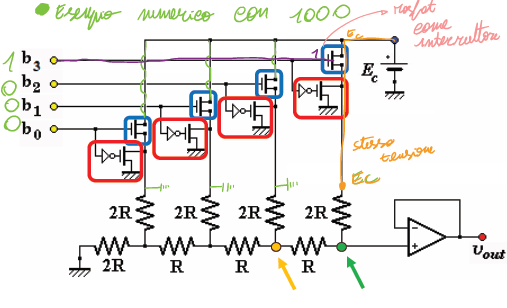
\includegraphics[scale = 1]{DAC a scala di resistenze 4 bit 1000.PNG}
\end{figure}

\newpage 

In questo caso numerico 1000: 

{
    \Large 
    \begin{equation}
        \begin{split}
        v_{out} 
        &= 
        \frac{E_c}{2^{4}}
        \left( 
            2^{3} b_3 
            +
            2^{2} b_2
            +
            2^{1} b_1
            +
            2^{0} b_0
        \right)
        \\ 
        &= 
        \frac{E_c}{2^{4}}
        \left( 
            2^{3} \cdot 1 
            +
            2^{2} \cdot 0
            +
            2^{1} \cdot 0
            +
            2^{0} \cdot 0
        \right)
        \\
        &= 
        \frac{E_c}{2^{4}} 
        \cdot
        2^{3}
        \\ 
        &= 
        \frac{E_c}{2} [V]
        \end{split}
    \end{equation}
}

\newpage 

\subsection{Half- flash ADC - pro e contro}
\footnote{Slide della prof | SDME 3.Conversione AD e Convertitori - Parte III | pag 18 - 19 \\  
Appunti | 2025-04-01 | pag 2 }

Come l'architettura Flash ADC, bisogna elencare i pro e i contro dell'architettura Half-flash ADC. \newline 

Il punto di forza è sicuramente la forte riduzione dei componenti fisici per realizzare l'half-flash. \newline 

Se consideriamo un ADC a 8 bit, per un flash-ADC a 8 bit sono necessari:

{
    \Large 
    \begin{equation}
        \begin{cases}
            2^{8} \text{ resistori } = 256 \text{ resistori }
            \\ 
            2^{8} - 1 \text{ comparatori } = 255 \text{ comparatori }
        \end{cases}
    \end{equation}
}

Invece, realizzando un half-flash ADC con 2 flash-ADC, un flash-ADC a 4 bit ha bisogno di: 

{
    \Large 
    \begin{equation}
        \begin{cases}
            2^{4} \text{ resistori } = 16 \text{ resistori }
            \\ 
            2^{4} - 1 \text{ comparatori } = 15 \text{ comparatori }
        \end{cases}
    \end{equation}
}

Moltiplicando per due i componenti per un half-flash a 8 bit: 

{
    \Large 
    \begin{equation}
        \begin{cases}
            16 \text{ resistori } \cdot 2 = 32 \text{ resistori }
            \\ 
            15 \text{ comparatori } \cdot 2 = 30 \text{ comparatori }
        \end{cases}
    \end{equation}
}

Invece il punto a sfavore dell'architettura half-flash è quello dell'aumento del tempo di conversione, dovuto all'effetto dei due "passi" in successione, in modo seriale. \newline 

A causa di questa caratteristica, gli half-flash non sono indicati per applicazioni in tempo reale. \newline 

Il tempo di conversione è la somma di tutti questi tempi perchè le operazioni viste vanno eseguite in cascata. \newline 

Gli half-flash erano adatti per applicazioni che non richiedevano elevate frequenze di campionamento, essendo meno costosi dei flash ADC. \newline 

Il compromesso da scegliere è o avere una maggiore risoluzione o aspettare, quindi avere una velocità di conversione maggiore. \newline 

La scelta dell'architettura half-flash ADC va fatta se siamo dispositi ad aspettare di più, rispetto agli ADC flash, a causa del maggior tempo di conversione, per avere in cambio una maggior risoluzione. \newline 

\newpage

\section{Two-stage pipelined flash Adc}
\footnote{Slide della prof | SDME 3.Conversione AD e Convertitori - Parte III | pag 20 \\  
Appunti | 2025-04-01 | pag 2 - 3}

Con il miglioramento della tecnologia, si è riusciti ad aumentare la frequenza di lavoro degli half-flash ADC, 
introducendo i "pipelined". \newline 

Di seguito lo schema del two-stage pipelined flash ADC: 

\begin{figure}[h]
    \centering
    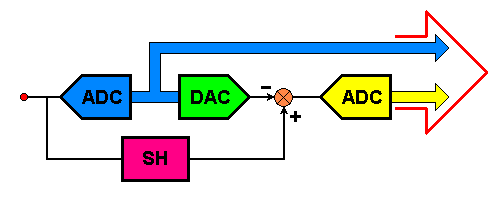
\includegraphics[scale = 1]{Two-stage pipelined flash ADC.png}
\end{figure}

Rispetto alle architetture ADC viste precedentemente, cioè quella flash e quella half-flash, 
questo tipo di architettura è intermedia tra le due. \newline 

Rispetto all'architettura half-flash: 

\begin{figure}[h]
    \centering
    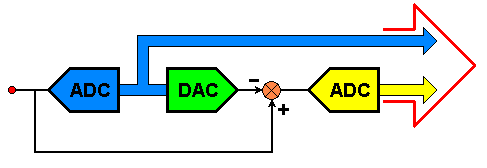
\includegraphics[scale = 0.6]{Half-flash ADC architettura.png}
\end{figure}


viene aggiunto un Sample and Hold (S \& H) supplementare: 
così facendo, una volta che il primo ADC (quello in blu) ha convertito un primo campione, 
esso può essere comandato a prelevare il campione successivo senza dover aspettare che gli altri blocchi terminino le proprie operazioni. \newline 

I tempi, rispetto all'architettura half-flash, diminuiscono visto che la modalità pipelined rende il primo ADC asincrono rispetto al resto dei blocchi circuitali. \newline 

Idealmente il DAC è istantaneo, nella realtà ha bisogno di tempo per assestarsi sulla tensione che deve emettere. \newline 

È un'architettura quasi parallela, perlopiù rimane seriale. \newline 

Il pro di utilizzare questa architettura è l'aumento del throughput (cioè la frequenza con cui si possono fornire i dati in uscita, e quindi della frequenza di campionamento) 
grazie alla strategia "pipeline". \newline 

Il contro è l'aumento della complessità circuitale di uno o più S \& H. \newline  


\newpage

\section{Multi-stage pipelined flash Adc}
\footnote{Slide della prof | SDME 3.Conversione AD e Convertitori - Parte III | pag 21 \\  
Appunti | 2025-04-01 | pag 3}

Aggiungendo più stadi al two-stage pipelined flash ADC si possono aumentare il numero di bit di risoluzione, ma diventa più complicato il circuito. \newline 

Di seguito uno schema di un Multi-stage pipelined flash Adc: 

\begin{figure}[h]
    \centering
    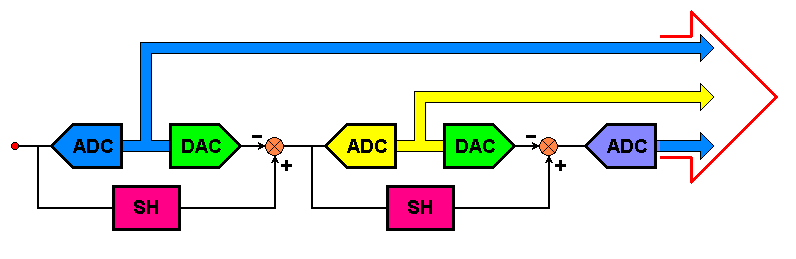
\includegraphics[scale = 0.7]{Multi-stage pipelined flash Adc.png}
\end{figure}

In figura una configurazione pipelined a 12 bit con i seguenti componenti: 

\begin{itemize}
    \item 3 ADC a 4 bit 
    \item 2 DAC 
    \item 2 S \& H
\end{itemize}

Rispetto al caso del two-stage pipelined flash ADC, bisogna aggiungere un altro S \& H, quindi il tempo di Hold dell'S \& H 
è molto importante. \newline 

I pro di questo tipo di architettura è l'ulteriore aumento del "throughput" rispetto all'architettura Two-stage pipelined flash Adc, 
e la riduzione di complessità rispetto a un flash ADC di uguale risoluzione. \newline 


Il contro è l'aumento del tempo di latenza a causa dei suoi tanti stadi di conversione. \newline 

Alche è consigliato questo tipo di architettura per applicazioni offline e non in tempo reale. \newline 

\newpage

\section{Convertitore a successive approssimazioni "SAR ADC"}
\footnote{Slide della prof | SDME 3.Conversione AD e Convertitori - Parte III | pag 23 - 24 \\  
Appunti | 2025-04-01 | pag 4 }

I convertitori a successive approssimazioni sono una famiglia di convertitori che segue un approccio opposto a quello visto finora. \newline

Se nei flash avevamo tanti comparatori per confrontare la tensione in ingresso con tutte le frontiere tra gli intervalli di quantizzazione, 
nei SAR ADC è presente un unico comparatore che confronta in maniera ciclica la tensione da convertire. \newline 

Ipotizzando di avere un campo di misura unipolare come in figura: 

\begin{figure}[h]
    \centering
    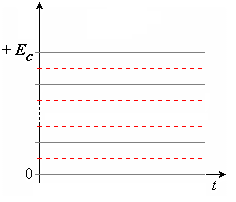
\includegraphics[scale = 1]{Campo unipolare.png}
\end{figure}

che va da 0 a $+E_c$ volt, suddiviso in un certo numero di intervalli uguali, si può realizzare un convertitore ad approssimazioni successive ad 8 bit come in figura: 

\begin{figure}[h]
    \centering
    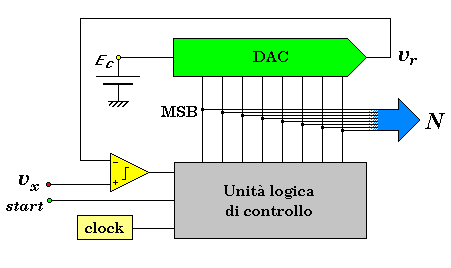
\includegraphics[scale = 1]{SAR ADC a 8 bit.png}
\end{figure}

Un SAR ADC è composto dai seguenti elementi: 

\begin{itemize}
    \item un campione di fem che eroga una tensione $E_c$ 
    \item un convertitore D/A (quello colorato in verde) a 8 bit che eroga una tensione $v_r$ 
    \item un comparatore (quel triangolino in basso a sinistra della figura) che confronta la tensione generata dal DAC, cioè $v_r$ con la tensione $v_x$ che vogliamo convertire 
    \item un'unità logica di controllo (o abbreviata con ULC) che ha la capacità di determinare il valore di ciascuna delle, in questo caso, 8 linee 
    \item un clock che ha il compito di cadenzare lo svolgimento di un processo ciclico, che inizia quando viene mandato un segnale di start alla ULC 
\end{itemize}

Il metodo del SAR ADC è un metodo iterativo, in cui, ogni colpo di clock, si porta il segnale nel DAC. \newline 

\newpage 

\subsection{SAR ADC: funzionamento "ideale"}
\footnote{Slide della prof | SDME 3.Conversione AD e Convertitori - Parte III | pag 25 - 29 \\  
Appunti | 2025-04-01 | pag 4 - 5 }

Per la spiegazione, consideriamo un convertitore SAR a 4 bit, quindi $2^{4} = 16$ intervalli come in figura: 

\begin{figure}[h]
    \centering
    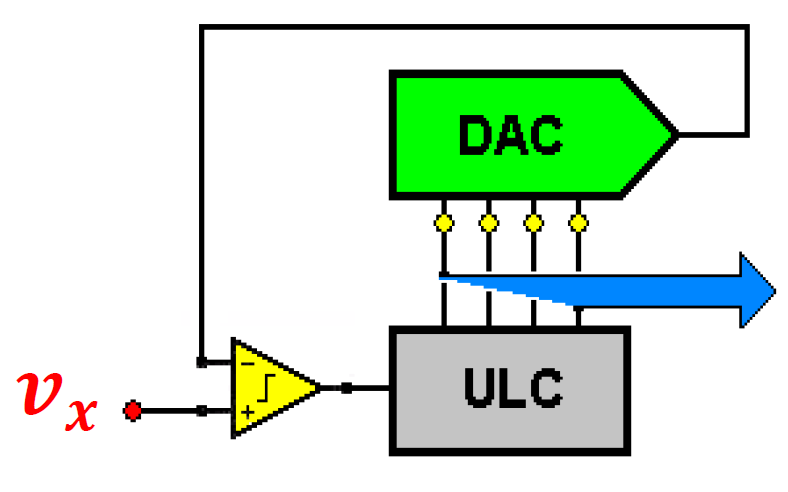
\includegraphics[scale = 0.4]{SAR ADC a 4 bit.png}
\end{figure}

Supponiamo che la tensione $v_x$ che deve essere convertita: 

\begin{figure}[h]
    \centering
    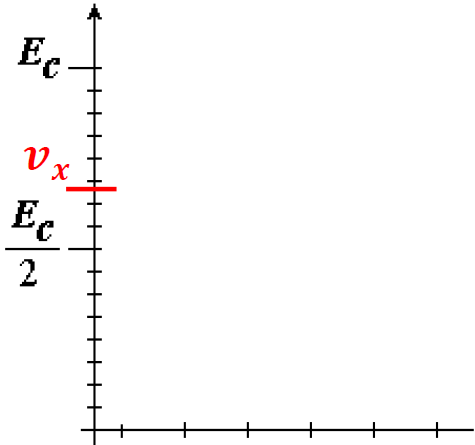
\includegraphics[scale = 0.4]{SAR ADC 1 step v_x.PNG}
\end{figure}

abbia il livello indicato in rosso, e cada dunque in quell'intervallo e sia superiore alla tensione $\frac{E_c}{2}$. \newline 

Quando si dà lo start (step molto importante che servirà anche nelle prossime architetture, perchè il processo di conversione inizia dal segnale di start) 
il primo passo che l'ULC esegue consiste nel portare ad 1 il bit più significativo che è in ingresso al DAC come si vede in figura: 

\begin{figure}[h]
    \centering
    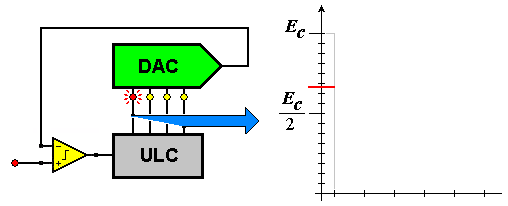
\includegraphics[scale = 1]{SAR ADC 2 step v_x.PNG}
\end{figure}

Il DAC "reagisce" a questa situazione portando in uscita una tensione che è metà della tensione di $E_c$ che è al suo ingresso perchè $v_x$ è minore di $E_c$ : 

\begin{figure}[h]
    \centering
    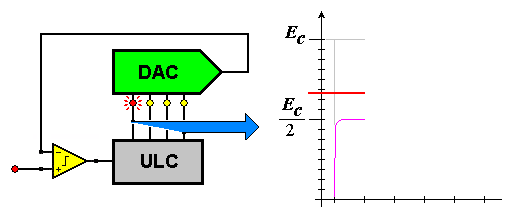
\includegraphics[scale = 1]{SAR ADC 3 step v_x.PNG}
\end{figure}

\newpage 

Il comparatore confronta la tensione $v_x$ con il valore di uscita dal DAC: 
dal confronto, si vede che $v_x$ è maggiore di $\frac{E_c}{2}$: 

\begin{figure}[h]
    \centering
    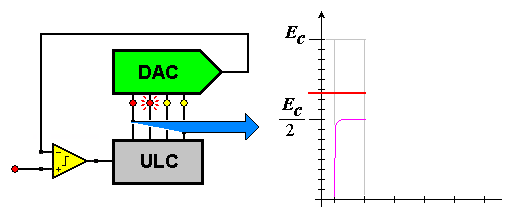
\includegraphics[scale = 1]{SAR ADC 4 step v_x.PNG}
\end{figure}

Quindi viene portato ad 1 anche il secondo ingresso del DAC e aumenta di $\frac{E_c}{4}$ la tensione di $\frac{E_c}{2}$: 

\begin{figure}[h]
    \centering
    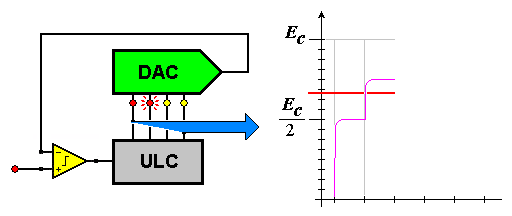
\includegraphics[scale = 1]{SAR ADC 5 step v_x.PNG}
\end{figure}

Ma la configurazione 1100 porta la tensione di uscita del DAC a $\frac{3}{4} E_c$ che è maggiore di $v_x$. \newline 

Allora, si spegne il secondo bit, si accende il terzo bit portando la tensione a $\frac{E_c}{2} + \frac{E_c}{8}$: 

\begin{figure}[h]
    \centering
    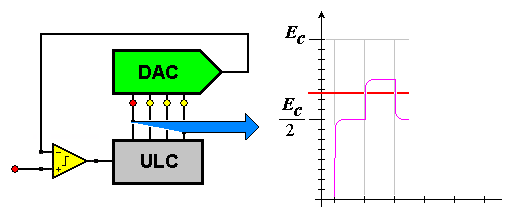
\includegraphics[scale = 1]{SAR ADC 6 step v_x.PNG}
\end{figure}

\newpage 

Si continua il processo che abbiamo indicato: 

\begin{figure}[h]
    \centering
    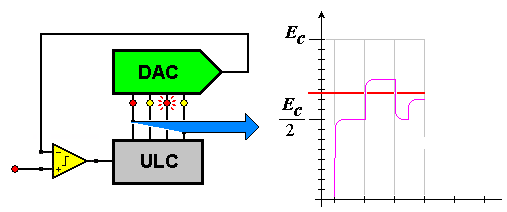
\includegraphics[scale = 1]{SAR ADC 7 step v_x.PNG}
\end{figure}

finché questi due casi si ripeteranno ciclicamente: 

\begin{figure}[h]
    \centering
    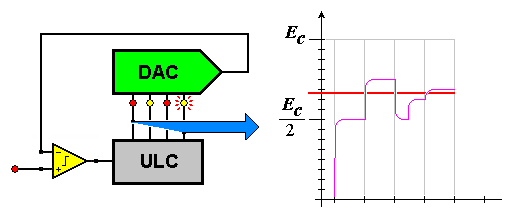
\includegraphics[scale = 1]{SAR ADC 8 step v_x.PNG}
    \\ 
    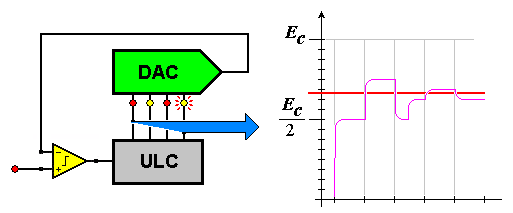
\includegraphics[scale = 1]{SAR ADC 9 step v_x.PNG}
\end{figure}

\newpage 

Quando la tensione dal DAC va sopra e sotto $v_x$, si dice che la tensione dal DAC si è stabilizzata. \newline 

Spetta poi all'ULC decidere come approssimare la tensione $v_x$. \newline  

Se starà sopra, si approssimerà $v_x$ per eccesso, se starà sotto, si approssimerà $v_x$ per difetto, 
quindi bisgognerà scegliere se porre a 1 o a 0 il LSB. \newline 

La scelta 

\begin{figure}[h]
    \centering
    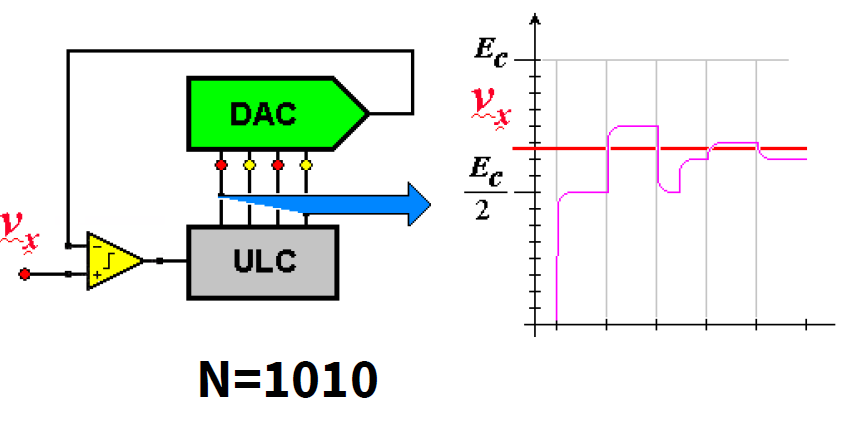
\includegraphics[scale = 0.5]{SAR ADC step v_x finale.PNG}
\end{figure}

è una scelta possibile di $v_x$. \newline 

\newpage 

\subsection{SAR ADC: pro e contro}
\footnote{Slide della prof | SDME 3.Conversione AD e Convertitori - Parte III | pag 30 \\  
Appunti | 2025-04-01 | pag 5 }

Usando un solo comparatore e un DAC, con una tecnica ciclica di successive approssimazioni, si è individuato l'intervallo in cui si trova 
la tensione $v_x$, con una circuiteria relativamente semplice. \newline 

Il processo è ciclico, iterativo, e non si svolge in un solo colpo di clock come nel flash ADC: 
occorrono alcuni $\mu s$ per convertire un certo numero di bit. \newline 

Quindi è molto più lento di un flash ma ha risoluzione più elevata e incertezza di quantizzazione molto più piccola. \newline 

Le applicazioni tipiche sono le registrazioni audio. \newline

Le caratteristiche tipiche di un SAR ADC sono quelle di avere una risoluzione dai 16 ai 18 bit con una relativa lentezza di processione, circa 2 $\mu s$ per un SAR ADC a 16 bit. \newline 

\newpage 

\section{Cause di incertezza nei convertitori}
\footnote{Slide della prof | SDME 3.Conversione AD e Convertitori - Parte III | pag 31 - 32 \\  
Appunti | 2025-04-01 | pag 5 }

In questa sezione si elencheranno le cause di incertezza nelle architetture dei convertitori ADC studiate. \newline 

\textbf{Flash ADC} 

\begin{itemize}
    \item Incertezza di quantizzazione, che affligge tutti i convertitori 
    \item stabilità del campione di fem 
    \item la stabilità dei valori nominali dei singoli resistori 
    \item errori di linearità dovuta alla ripartizione dei valori di tensione tra i vari resistori 
    \item offset dei comparatori, che affligge soprattutto le misure di tensioni piccole 
\end{itemize}

\textbf{Semi-flash ADC} 

\begin{itemize}
    \item Incertezza di quantizzazione 
    \item stabilità dei campioni di fem contenuti nei convertitori ADC 
    \item errori di linearità del convertitore DAC 
    \item stabilità del campione fem del DAC 
    \item comportamento della giunzione che deve operare la differenza tra le tensioni
\end{itemize}

In genere, le ultime quattro cause, sono considerate trascurabili rispetto all'incertezza di quantizzazione, che è la principale causa di incertezza sia nei flash che negli Half-flash ADC. \newline 

\textbf{SAR ADC} 

\begin{itemize}
    \item Incertezza di quantizzazione 
    \item stabilità del campione di fem, che diventa instabile se la temperatura non è nel range in cui è stato tarato il fem 
    \item linearità del DAC 
    \item offset e la sensibilità del comparatore
\end{itemize}


\newpage 

\section{Convertitore ad inseguimento}
\footnote{Slide della prof | SDME 3.Conversione AD e Convertitori - Parte III | pag 33 \\  
Appunti | 2025-04-01 | pag 5 - 6 }

Un altro tipo di architettura di ADC è quella del convertitore ad inseguimento. \newline 

Partendo dall'architettura del SAR ADC: 

\begin{figure}[h]
    \centering
    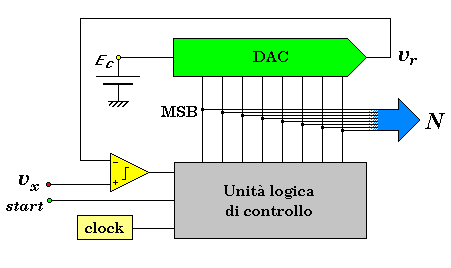
\includegraphics[scale = 0.8]{SAR ADC a 8 bit.png}
\end{figure}

si può considerare un'ulteriore famiglia di convertitori, cioè quelli ad inseguimento. \newline 

Sostituendo l'unità logica di controllo con un contatore up-down: 

\begin{figure}[h]
    \centering
    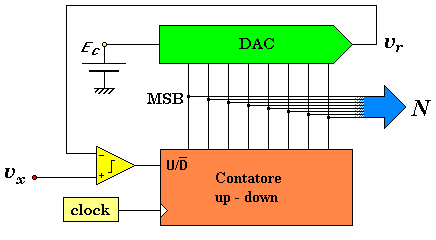
\includegraphics[scale = 0.8]{Convertitore up-down.png}
\end{figure}

Ad ogni impulso di clock, il convertitore aggiorna il contatore, cioè il contenuto del suo registro, 
incrementandolo o decrementandolo di 1 dello stato della linea $U / \overline{D}$. \newline 

Il DAC ha in ingresso il valore totalizzato dal contatore. \newline 

\newpage 

\subsection{Principio di funzionamento}
\footnote{Slide della prof | SDME 3.Conversione AD e Convertitori - Parte III | pag 34 - 35 \\  
Appunti | 2025-04-01 | pag 6 | 2025-04-02 | pag 2 }

Vediamo cosa accade quando in ingresso a questo convertitore mettiamo una tensione non campionata da S \& H, ma con andamento di tipo analogico. \newline 

La tensione $v_x$ ha il seguente andamento: 

\begin{figure}[h]
    \centering
    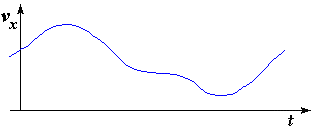
\includegraphics[scale = 0.8]{Tensione analogica in ingresso al convertitore ad inseguimento.png}
\end{figure}

All'inizio il contatore ha uscita nulla, quindi il compratore che confronta la tensione che esce dal DAC con quella in ingresso $v_x$ 
avrà sempre uscita a livello alto. \newline 

Il contatore continuerà ad incrementare il proprio valore in uscita di 1 unità ogni colpo di clock. \newline 

La tensione in uscita dal DAC sale con un andamento a gradinata, 
fino a che non incrocia il valore della tensione analogica. \newline 

Adesso che il segnale $v_r$ si è agganciato a quello di $v_x$, $v_r$ varia di +1 o -1 in base l'andamento del segnale $v_x$: 

\begin{figure}[h]
    \centering
    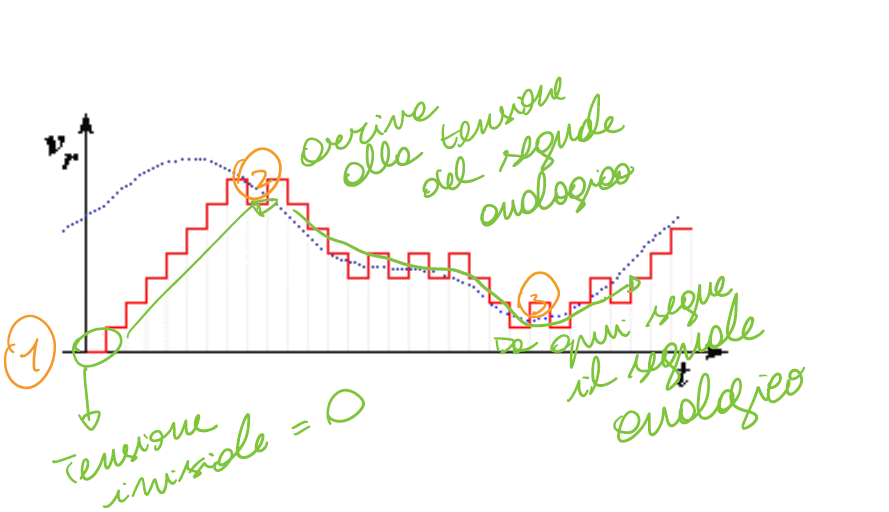
\includegraphics[scale = 0.6]{andamento vr rispetto a vx.PNG}
\end{figure}

per questo motivo, nei convertitori ad inseguimento è consigliato un segnale analogico che non si modifica tanto in un breve periodo. \newline 

Il fatto di cambiare un solo bit alla volta, permette di avere una latenza estremamente bassa e una buona risoluzione perchè deriva dai SAR ADC. \newline 

La tecnica di alzare la frequenza di campionamento diventa strategica per ridurre il rumore di quantizzazione. \newline 

\newpage 

\subsection{Filtro numerico BB}
\footnote{Slide della prof | SDME 3.Conversione AD e Convertitori - Parte III | pag 36}

In un convertitore SAR convenzionale, il tempo di conversione è relativamente lungo. \newline 

Quindi la frequenza di campionamento $f_c$ non può essere molto elevata. \newline 

Come si vede dalla figura: 

\begin{figure}[h]
    \centering
    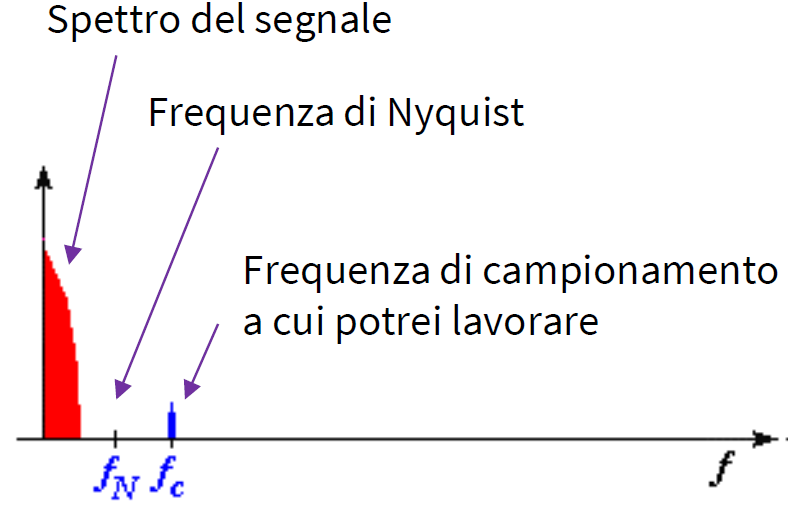
\includegraphics[scale = 0.4]{spettro dei segnali in un SAR ADC parte 1.PNG}
\end{figure}

$f_c$ sarà superiore alla frequenza di Nyquist $f_N$, ma non troppo alta. \newline 

Come abbiamo studiato a Teoria dei segnali con il mitico Chiaraluce, quando vado a campionare, 
ovvero si fa la convoluzione tra gli spettri, la prima replica dello spettro ha una frequenza minima pari a $f_c - B$: 

\begin{figure}[h]
    \centering
    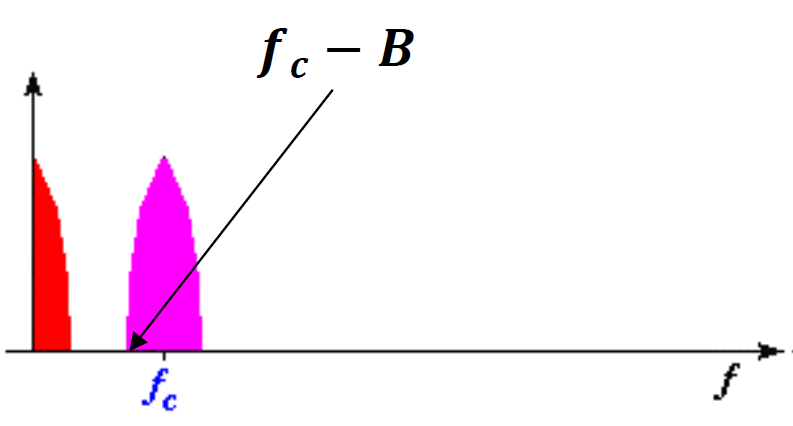
\includegraphics[scale = 0.4]{spettro dei segnali in un SAR ADC parte 2.PNG}
\end{figure}

Se si vuole ricostruire il segnale di banda base (BB) dal segnale campionato, eliminando le repliche, 
il filtro BB ha requisiti molto stringenti perchè deve essere molto ripido: 

\begin{figure}[h]
    \centering
    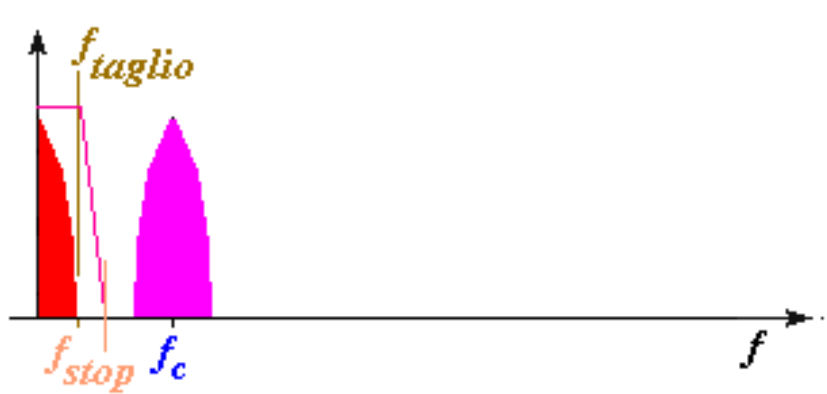
\includegraphics[scale = 0.4]{spettro dei segnali in un SAR ADC parte 3.PNG}
\end{figure}

Invece, se si campiona un segnale ad una frequenza $f_c$ maggiore, ci sarebbe un "buco" in frequenza maggiore tra il segnale campionato (quello viola) e il segnale in BB (quello rosso). \newline 

\newpage 

\subsection{Filtro numerico BB con convertitore ad inseguimento}
\footnote{Slide della prof | SDME 3.Conversione AD e Convertitori - Parte III | pag 37 \\  
Appunti | 2025-04-02 | pag 3 }

Invece, campionando con un convertitore ad inseguimento, la frequenza di campionamento $f_c$ è nettamente più alta rispetto alla frequenza di Nyquist $f_N$, 
quindi c'è più spazio in frequenza tra la frequenza massima del segnale in BB e il segnale campionato. \newline 

Allora si può realizzare un filtro meno ripido rispetto al caso del SAR ADC. \newline 

Con le seguenti figure, si riassume quello che succede in frequenza con un convertitore ad inseguimento: 

\begin{figure}[h]
    \centering
    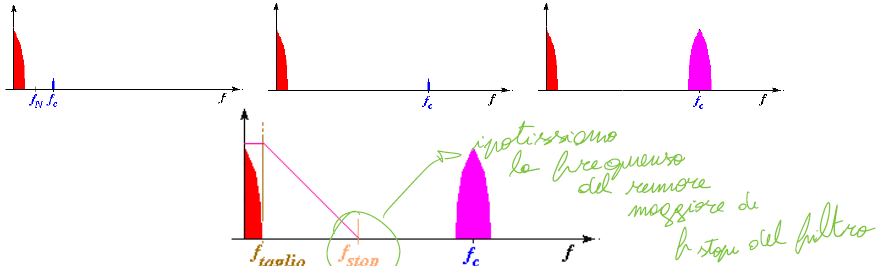
\includegraphics[scale = 0.6]{spettro dei segnali in un convertitore ad inseguimento.PNG}
\end{figure}

\newpage 

\subsection{Rumore di quantizzazione}
\footnote{Slide della prof | SDME 3.Conversione AD e Convertitori - Parte III | pag 38 - 39 \\  
Appunti | 2025-04-02 | pag 3 }

Per errore di quantizzazione si intende la differenza tra il valore della tensione da convertire (cioè il segnale reale) 
e il valore quantizzato che lo rappresenta. \newline 

Le considerazioni svolte saranno svolte quando il segnale campionato è arrivato a regime, trascurando il transitorio iniziale. \newline 

Considerano il segnale $\delta q$ come il segnale di rumore: 

\begin{figure}[h]
    \centering
    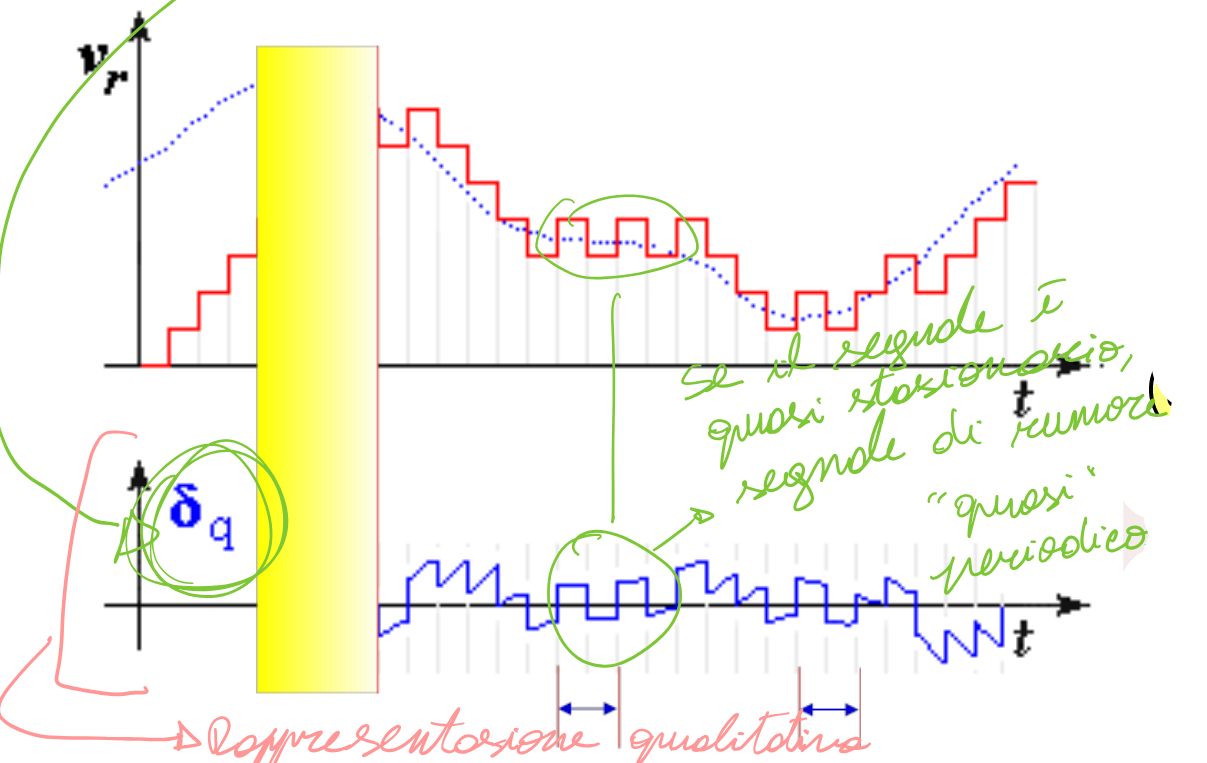
\includegraphics[scale = 0.6]{errore di quanrizzazione in un convertitore ad inseguimento.png}
\end{figure}

cioè la differenza tra segnale quantizzato e reale, che possiamo chiamare anche come rumore di quantizzazione. \newline  

Che frequenza ha $\delta q$ ? \newline 

Il rumore di quantizzazione ha un periodo che non supera il doppio del periodo di campionamento: 
o è uguale al periodo di campionamento nel transitorio, o è uguale al doppio nei tratti di segnale a regime. \newline 

Vedendolo in frequenza, se il rumore di quantizzazione ha un periodo: 

{
        \Large 
        \begin{equation}
            \begin{split}
            T_{noise} &\leq 2 T_c 
            \\
            &\updownarrow 
            \\
            f_{noise} &\ge \frac{f_c}{2}
            \end{split}
        \end{equation}
}

Quindi si può inserire un filtro numerico in uscita all'ADC per attenuare il rumore di quantizzazione: 

\begin{figure}[h]
    \centering
    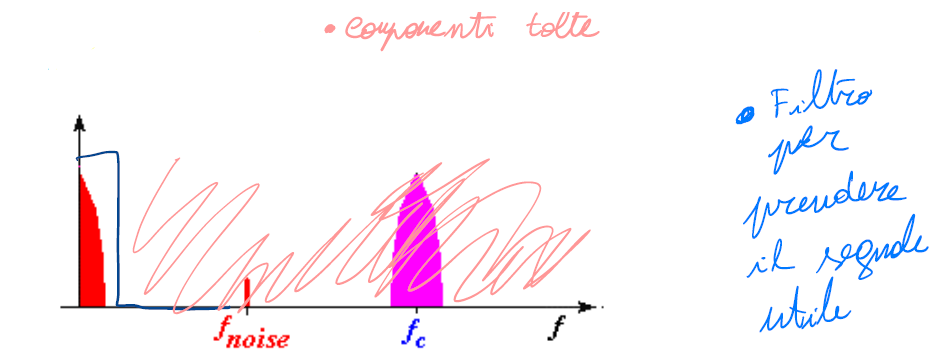
\includegraphics[scale = 0.6]{filtro per recuperare il segnale in BB anche se esiste rumore di quantizzazione.PNG}
\end{figure}

\newpage 

L'intensità del rumore di quantizzazione (o rumore di campionamento) non ha effetto, visto che lo si può filtrare, 
quindi si possono realizzare anche dei convertitori grossolani, in cui tale rumore non sia trascurabile, 
perchè comunque lo si può filtrare: questo è il principio impiegato dai convertitori sigma-delta. \newline 

\newpage 

\section{Sigma-Delta $\Sigma - \Delta$}
\footnote{Slide della prof | SDME 3.Conversione AD e Convertitori - Parte III | pag 40 - 41 \\  
Appunti | 2025-04-02 | pag 3 - 5}

Lo schema a blocchi di un convertitore Sigma-Delta:

\begin{figure}[h]
    \centering
    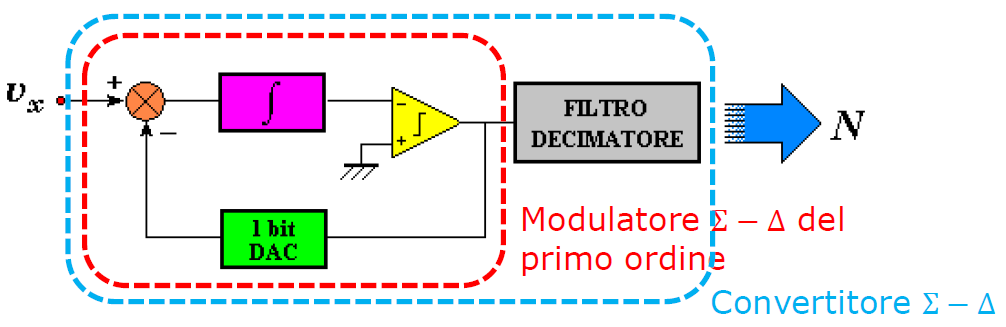
\includegraphics[scale = 0.5]{Schema a blocchi convertitore Sigma Delta.PNG}
\end{figure}

Il blocco viola è un blocco integratore, che integra il residuo tra $v_x$ e quello che esce dal DAC. \newline 

Il concetto di questo convertitore è quello di codificare la variazione che il segnale esibisce tra campioni consecutivi. \newline 

Come si vede dallo schema del Sigma-Delta, è presente un comparatore (triangolo giallo), 
ma sulla retroazione è presente un DAC ad un solo bit, quindi grossolano. \newline 

Il filtro decimatore (quello in grigio) ha il compito di eliminare il rumore di quantizzazione in uscita. \newline 

Con questa architettura, si possono avere frequenze di campionamento molto alte, risoluzioni elevate con prezzi contenuti. \newline 


I convertitori Sigma-Delta sono quelli più usati oggigiorno, in particolare nell'ambito delle telecomunicazioni. \newline 

Sono basati su uno schema di principio che prevede il ricorso alle operazioni di sovra-campionamento (oversampling), 
quantization noise shaping, filtraggio digitale e decimazione. \newline 

Possiamo visualizzare i diversi schemi di architetture rispetto al rumore in frequenza con questi casi: 

\begin{figure}[h]
    \centering
    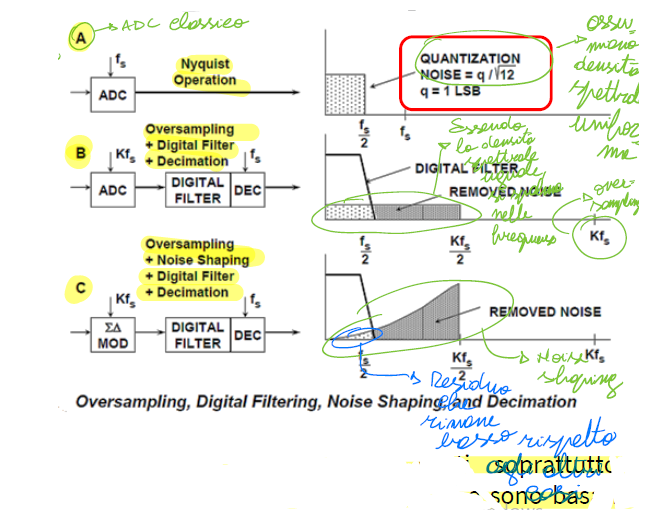
\includegraphics[scale = 0.8]{contributi dei componenti del sigma delta in frequenza.PNG}
\end{figure}

\newpage 

Il noise shaping è una tecnica che solo i circuiti digitali possono fare. \newline

In pratica il noise shaping prende la densità spettrale del rumore e poi lo spalma in tutta la banda. \newline 

In commercio, si possono trovare convertitori che integrano il campionatore, cioè il Sample and Hold. \newline 

\newpage 

\section{Limiti dei convertitori}
\footnote{Slide della prof | SDME 3.Conversione AD e Convertitori - Parte III | pag 43 - 47 \\  
Appunti | 2025-04-02 | pag 6 - 7}

Ogni convertitore è soggetto ad errori di conversione e limiti che derivano dalla quantizzazione della tensione: rumore elettrico, altre imperfezioni e non idealità dei componenti. \newline 

L'errore di quantizzazione può essere calcolato e limitato, ma mai del tutto eliminato. \newline 

Errori e limitazioni dovuti a non idealità sono propri di ogni specifico convertitore: 
una volta misurato l'errore, si può correggere l'effetto in seguito alla misura. \newline 

Un ADC, per ogni valore convertito, associa un errore limitato, pari a $\pm \frac{1}{2}$ LSB (Least Significant  Bit). \newline 

Lo scarto tra il valore d'ingresso e il valore digitalizzato presenta una distribuzione uniforme, perchè si considera ogni valore equiprobabile in quell'intervallo, 
chiamato passo di quantizzazione, 
la cui larghezza è importante per definire l'incertezza di quantizzazione. \newline 

Il passo di quantizzazione dell'ADC è largo $\Delta v$ sulla scala dei possibili valori di ingresso ed è largo una unità di conteggio o 1 LSB in numeri sulla scala dei valori digitali di uscita. \newline 

Oltre all'errore intrinseco di quantizzazione, un ADC presenta una caratteristica di conversione che differisce da quella ideale, 
dovuto principalmente da: 

\begin{itemize}
    \item errore di offset 
    \item errore di guadagno 
    \item errore di non linearità
\end{itemize}

Se si considera un ADC unipolare ideale, questa è la relazione tra ingresso analogico e i codici in uscita, e l'errore di quantizzazione: 

\begin{figure}[h]
    \centering
    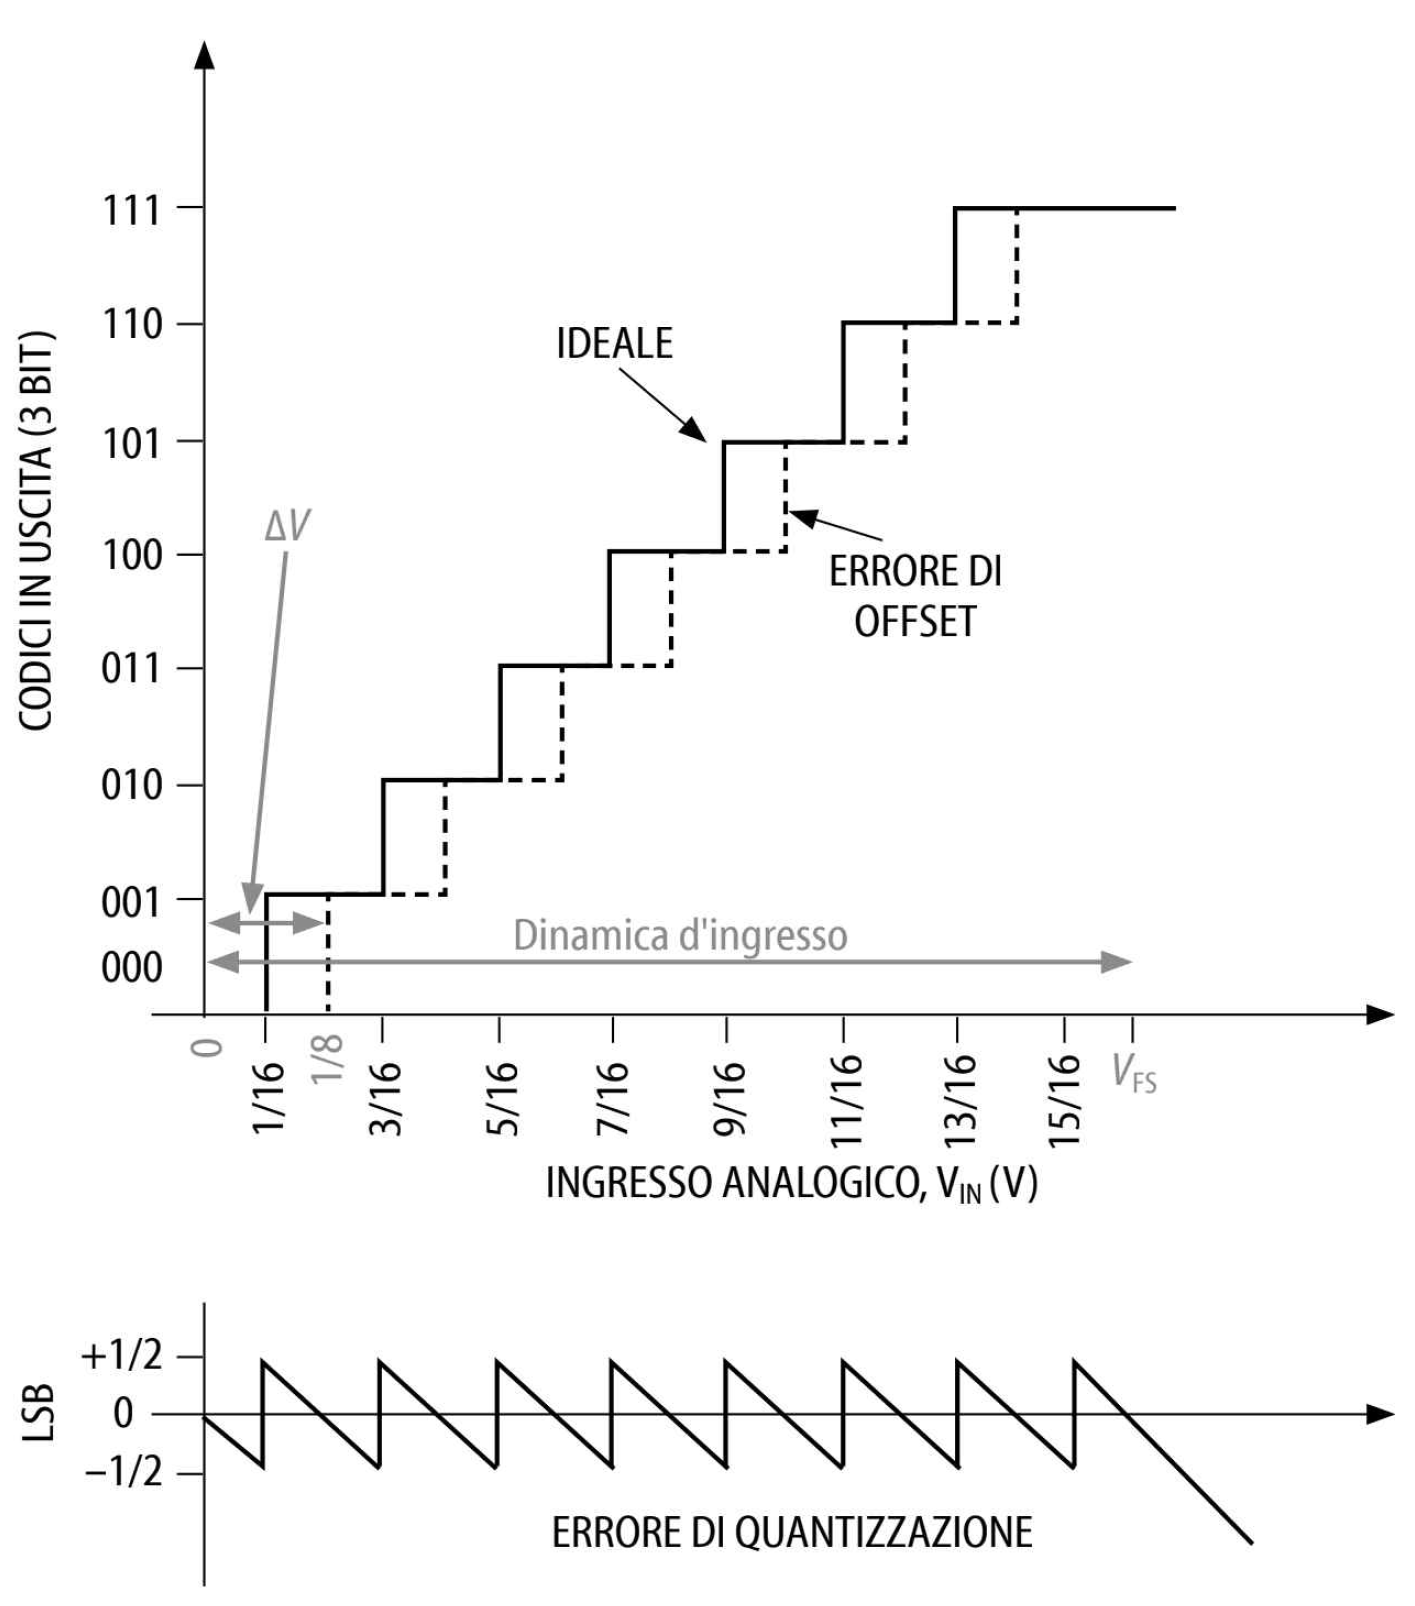
\includegraphics[scale = 0.2]{conversione di un ADC unipolare ideale ed errore di quantizzazione.png}
\end{figure}

L'errore di offset è definito come uno spostamento comune a tutti i codici, delle transizioni rispetto ai valori ideali delle tensioni, nella corrispondente caratteristica ideale. \newline 

Ciò comporta una traslazione secondo la direzione dell'asse delle ascisse di tutta la caratteristica ideale: 
può essere rilevato e dunque compensato con una semplice misura di zero, cioè misurare l'ADC senza un segnale di ingresso e diminuendo il valore in uscita dopo questa misura. \newline 

Invece, per l'errore di guadagno si intende una variazione della pendenza della caratteristica di trasferimento reale rispetto a quella ideale. \newline 

Si può notare il contributo dell'errore di guadagno in questa figura: 

\begin{figure}[h]
    \centering
    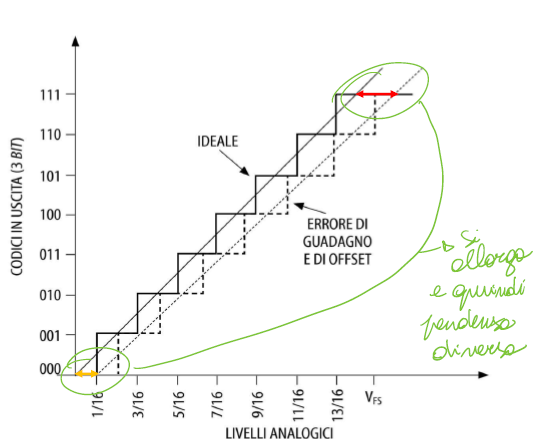
\includegraphics[scale = 0.6]{effetto dell'errore di guadagno nei convertitori.PNG}
\end{figure}

Anche questo tipo di errore può essere compensato, ma richiede una misura di taratura, e quindi un confronto con un sistema di misura più accurato. \newline 

Un altro problema citato dei convertitori è l'errore di non linearità, che si traduce in una larghezza reale del passo di quantizzazione che differisca da quella ideale. \newline 

Come si nota dalle seguenti figure: 

\begin{figure}[h]
    \centering
    \includegraphics[scale = 0.6]{non linearità negli ADC.PNG}
\end{figure}

la non linearità rende i passi non omogenei e non proporzionali. \newline 

\newpage 

\section{Velocità, risoluzione, accuratezza}
\footnote{Slide della prof | SDME 3.Conversione AD e Convertitori - Parte III | pag 48 - 50 \\  
Appunti | 2025-04-02 | pag 8 | 2025-04-04 | pag 2 }

Per la maggior parte delle applicazioni, le due più importanti caratteristiche dei convertitori A/D sono la velocità e la risoluzione. \newline 

I parametri di interesse di un ADC sono: 

\begin{itemize}
    \item la massima frequenza di campionamento $f_{C, MAX}$ in [$\frac{Sa}{s}$] (si legge Samples per second, cioè campioni ogni secondo) o [Hz]
    \item certe volte viene impiegato l'inverso della frequenza di campionamento, cioè il minimo periodo di campionamento $T_{C, MIN}$ che si misura in [s]
    \item la risoluzione, che dipende dallo strumento, generalmente la grandezza da misurare è la tensione quindi la risoluzione $\Delta V$ si misura in [V] 
    \item l'accuratezza o incertezza di misura che denotiamo con u(V) (dall'inglese uncertainty di V) misurata in [V]
\end{itemize}


Quando si va a scegliere un ADC disponibile nel mercato, la velocità dell'ADC si deve bilanciare con la risoluzione e bisogna trovare un giusto compromesso tra i due 
(come al solito in ingegneria, non puoi avere la moglie ubriaca e la botte piena). \newline 

La velocità massima da da garantire è quella data dal teorema del campionamento. \newline 

La risoluzione di un metodo di misura o di uno strumento è, in genere, la capacità di distinguere o separare stati diversi del misurando, ovvero per un convertitore è il suo passo di quantizzazione. \newline 

\begin{tcolorbox}
In questo corso, le misure saranno sempre riportate in tensione    
\end{tcolorbox}

Riferendosi alla tensione, si parla di risoluzione (dimensionale) $\Delta V$ [V] e di risoluzione adimensionale $\delta$. \newline 

La dinamica di misura (o dinamica analogica) o dinamica di ingresso di un ADC (viene indicata con la lettera D), 
è l'intervallo di valori di tensione analogica che il convertitore riesce a trasformare correttamente in valori numerici. \newline 

La dinamica di uscita di un ADC è l'insieme dei valori numerici possibili in uscita da un convertitore A/D. \newline 

L'ADC quantizza l'uscita digitale su N diversi valori numerici che sono solitamente contati con i numeri interi da 0 a N-1. \newline 

Se la conversione A/D avviene con uscita codificata a n bit, allora: 

{
    \Large 
    \begin{equation}
        \begin{split}
        N &= 2^{n} 
        \\
        &\updownarrow
        \\
        n &= \log_{2}N
        \end{split}
    \end{equation}
}

Se l'ADC o lo strumento è lineare e opera su una dinamica D con N livelli di discretizzazione, la risoluzione dimensione $\Delta V$ è: 

{
    \Large 
    \begin{equation}
        \Delta V = \frac{D}{N}
    \end{equation}
}

Per alcuni strumenti di misura o per quegli ADC con dinamica esclusivamente unipolare, 
il termine dinamica D è a volte sostituito da portata P dello strumento. \newline 

Nei casi unipolari: 

{
    \Large 
    \begin{equation}
        \begin{split}
        D &= P
        \\ 
        &\downarrow
        \\ 
        \Delta V &= \frac{P}{N}      
        \end{split}
    \end{equation}
}

Nei casi bipolari: 

{
    \Large 
    \begin{equation}
        \begin{split}
        D &= 2P
        \\ 
        &\downarrow
        \\ 
        \Delta V &= \frac{2P}{N}      
        \end{split}
    \end{equation}
}

La risoluzione adimensionale è definita analiticamente come il reciproco del numero di livelli digitali o di quantizzazione: 

{
    \Large 
    \begin{equation}
        \delta = \frac{1}{N}
    \end{equation}
}

Spesso la risoluzione adimensionale è espressa anche come numero di bit n o come numero di cifre decimali M corrispondenti 
al numero di livelli di quantizzazione che il convertitore mette a disposizione, per cui si ha: 

{
    \Large 
    \begin{equation}
        \begin{split}
            n &= \delta_{(bit)} = \log_2 N 
            \\ 
            M &= \delta_{(cifre)} = \log_{10} N
        \end{split}
    \end{equation}
}

Quando le formule precedenti non forniscono un valore intero, si usa esprimere $\delta_{(bit)}$ alla prima cifra decimale, 
mentre $\delta_{(cifre)}$ si usa il valore approssimato al quarto di unità o alla mezza cifra decimale. \newline 

Affermare che un convertitore A/D ha M e $\frac{1}{2}$ cifre decimali è solamente indicativo del numero N di livelli: 
conoscendo M e $\frac{1}{2}$ cifre, si può solo inferire un intervallo di possibili valori per i livelli, ovvero: 

{
    \Large 
    \begin{equation}
        10^{M} < N < 10^{M+1}
    \end{equation}
}

\begin{tcolorbox}
    Un'altra regola aurea è leggere attentamente i datasheet degli strumenti e dei componenti, in modo da capire meglio come si comporta l'oggetto e i suoi parametri
\end{tcolorbox}

\newpage 

\section{Numero di cifre nei display dei DMM}
\footnote{Slide della prof | SDME 3.Conversione AD e Convertitori - Parte III | pag 51 \\  
Appunti | 2025-04-04 | pag 3}

Maggiore è il numero di digit del display di un DMM (Digital MultiMeter) e maggiore è la risoluzione. \newline 

La mezza cifra può essere solo 0 o 1. \newline 

Ad esempio, dato questo multimetro da banco: 

\begin{figure}[h]
    \centering
    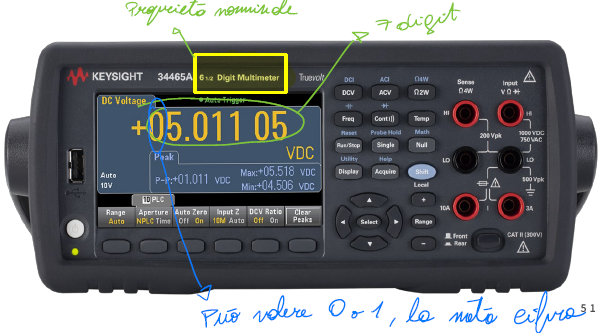
\includegraphics[scale = 0.8]{Misura da un DMM.PNG}
\end{figure}

Di seguito una tabelle di cifre presenti negli DMM: 

\begin{figure}[h]
    \centering
    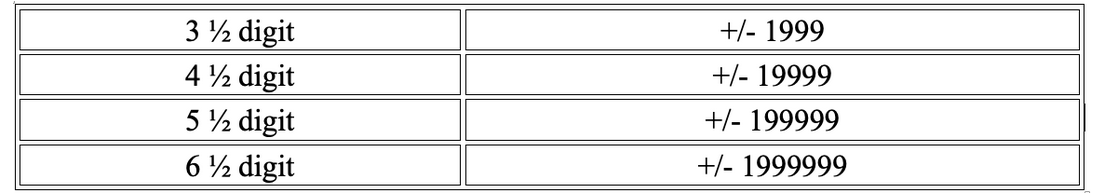
\includegraphics[scale = 0.5]{Tabellla cifre nei DMM.png}
\end{figure}

Tipicamente, se un DMM ha più di $4 \frac{1}{2}$ digit, è uno strumento da banco. \newline 

\newpage 

\section{Bit equivalenti - caso ideale}
\footnote{Slide della prof | SDME 3.Conversione AD e Convertitori - Parte III | pag 52 \\  
Appunti | 2025-04-04 | pag 3 - 4}

Consideriamo un convertitore A/D ideale a n bit e dinamica di ingresso D bipolare, estesa dunque ad un intervallo di valori possibili tra -D/2 e + D/2 per la tensione di ingresso. \newline 

Consideriamo un generico valore analogico di tensione s(t) in ingresso all'ADC di valore non noto a propri. \newline 

Esso è descrivibile come un processo aleatorio con distribuzione di probabilità delle ampiezze uniforme 
nell'intervallo $\left[ - \frac{D}{2}, + \frac{D}{2}\right]$ come si può vedere in figura: 

\begin{figure}[h]
    \centering
    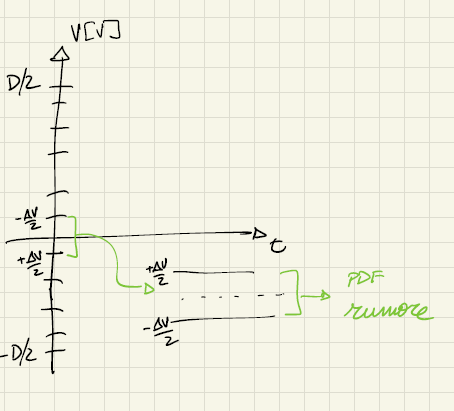
\includegraphics[scale = 0.8]{Varianza in un ADC ideale.PNG}
\end{figure}

\begin{tcolorbox}
    I calcoli svolti, quindi l'integrale del calcolo della varianza, sono omessi, ma sono gli stessi fatti a inizio corso considerando l'intervallo $\left[ - \frac{D}{2}, + \frac{D}{2}\right]$
\end{tcolorbox}

Pertanto, all'intervallo $\left[ - \frac{D}{2}, + \frac{D}{2}\right]$, è associata una varianza pari a: 

{
    \Large 
    \begin{equation}
        \sigma_S ^{2} = \frac{D^{2}}{12}
    \end{equation}
}

Essendo l'ADC ideale, esso opera una conversione A/D a n bit, affetta dal solo errore di quantizzazione. \newline 

Il passo di quantizzazione ha ampiezza: 

{
    \Large 
    \begin{equation}
        \Delta V = \frac{D}{N} = \frac{D}{2^{n}}
    \end{equation}
}

La varianza dell'errore di quantizzazione si può esprimere come: 

{
    \Large 
    \begin{equation}
        \begin{split}
        \sigma_q ^{2} 
        &= 
        \frac{\Delta V ^{2}}{12}
        \\ 
        &= 
        \frac{1}{12}
        \left(\frac{D}{2^{n}}\right)^{2}
        \\ 
        &= 
        \frac{D^{2}}{12}
        \left(\frac{1}{2^{n}}\right)^{2}
        \end{split} 
    \end{equation}
}

ovvero: 

{
    \Large 
    \begin{equation}
        \sigma_q ^{2} 
        = 
        \frac{\delta_s ^{2}}{2^{2n}}
    \end{equation}
}

Quindi, nel caso di un convertitore ideale, il numero di bit n si può esprimere come il 
rapporto di due varianze, che sono rispettivamente proporzionali alla potenza del segnale S e alla potenza 
del solo rumore di quantizzazione $N_q = N$, ovvero: 

{
    \Large
    \begin{equation}
        2^{2n} = \frac{\sigma_S ^{2}}{\sigma_q ^{2}} 
        = 
        \frac{S}{N_q} 
        = 
        SNR_{ideale}
    \end{equation}
}

\newpage 

\section{Bit equivalenti - caso reale}
\footnote{Slide della prof | SDME 3.Conversione AD e Convertitori - Parte III | pag 53 \\  
Appunti | 2025-04-04 | pag 5 | 2025-06-23 | pag 1, 3}


Considerando un convertitore reale a n bit, esso avrà più contributi di rumore, oltre a quello di quantizzazione del caso ideale. \newline

Rispetto al caso ideale, questa volta non indichiamo il modello, ma grazie al teorema del limite centrale (studiato nel corso di Teoria dei segnali), 
si può esprimere che per un fenomeno non ideale, la distribuzione di probabilità sarà di tipo gaussiano. \newline 

Si definisce numero di bit equivalenti di un convertitore reale, 
il numero di bit di un convertitore ideale in cui il rumore di sola quantizzazione è pari a quello complessivamente riscontrato nella conversione A/D: 

{
    \Large 
    \begin{equation}
        n_e 
        = 
        \frac{1}{2} \log_2 \left( \frac{\sigma_S ^{2}}{\sigma_{q, e} ^{2}}\right)
        = 
        \frac{1}{2} \log_2 \left( \frac{\sigma_S ^{2}}{\sigma_{N, A/D} ^{2}}\right)
    \end{equation}
}

e ne risulta che: 

{
    \Large 
    \begin{equation}
        n_e < n
    \end{equation}
}

\newpage 

\section{Bit equivalenti (ENOB)}
\footnote{Slide della prof | SDME 3.Conversione AD e Convertitori - Parte III | pag 54 - 56 \\  
Appunti | 2025-04-04 | pag 5}

Da: 
{
    \Large 
    \begin{equation}
        n_e < n
    \end{equation}
}

risulta che un convertitore a n bit può perdere un certo numero di bit di accuratezza a causa delle non idealità e dei rumori presenti. \newline 

Quindi, oltre ad avere un ADC di qualità con n bit elevati, 
una grande precauzione è quella di avere un segnale privo o con poco rumore, 
perchè diminuiranno le presetazioni dell'ADC. \newline 

Come ci dimostra il seguente grafico in cui mettere in relazione la SNR di un segnale dato in un ingresso ad un ADC: 

\begin{figure}[h]
    \centering
    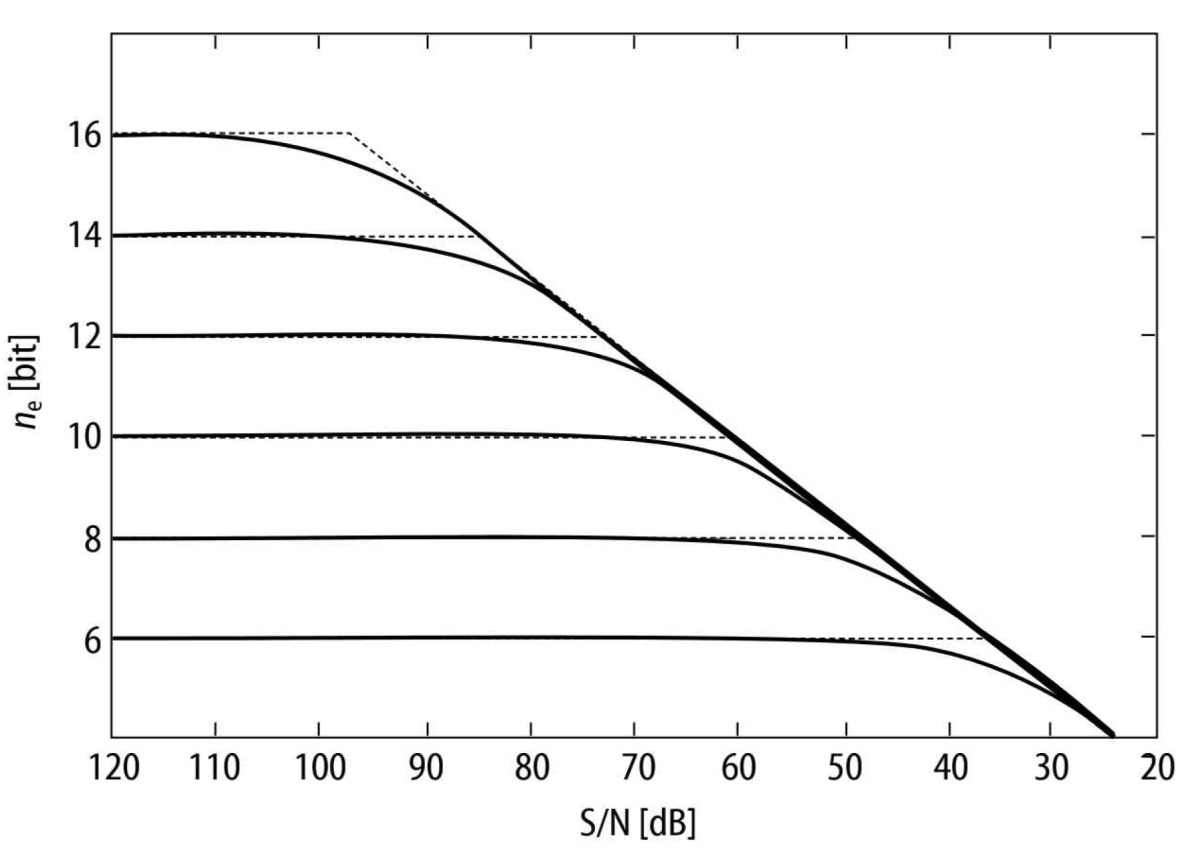
\includegraphics[scale = 0.6]{SNR e n bit di conversione.png}
\end{figure}

più SNR peggiora, minore saranno i bit di conversione dell'ADC. \newline 

Per un SNR che diminuisce (nella figura ci spostiamo a destra) di 6 dB (fattore 4), si perde 1 bit di conversione. \newline 

Dall'inglese, $n_e$ prende il nome di ENOB: Equivalent Number of Bits. \newline 

\newpage 

